\documentclass[12pt,a4paper]{article}
\usepackage[utf8]{inputenc} % For UTF-8 encoding
\usepackage{amsmath, amssymb} % For mathematical symbols
\usepackage{graphicx} % For including images
\usepackage{hyperref} % For clickable links
\usepackage{geometry} % For page margins
\usepackage{booktabs} % For nice tables
\usepackage{lipsum} % For dummy text
\usepackage{longtable}
\usepackage{algorithm}
\usepackage{algorithmic}
\usepackage[style=apa, sorting=nyt, backend=biber]{biblatex} % Use biber as the backend
\addbibresource{references.bib}

\setlength{\parindent}{0em}
% Page layout
\geometry{margin=1in}

% Hyperlink setup
\hypersetup{
    colorlinks=true,
    linkcolor=blue,
    filecolor=magenta,
    urlcolor=cyan,
    pdftitle={LaTeX Template},
    pdfpagemode=FullScreen,
}

% ######################## Title  Page ####################################
\title{Recurrent Deep Learning Models and its applications}
\author{Ngai Ho Wang}

\date{\today}

\begin{document}

\maketitle
% ######################## Title  Page ####################################

% ######################## table of content ###############################
\tableofcontents % Generate a table of contents                        
% ######################## table of content ###############################

\newpage
% ######################## Introduction ####################################
\section{Introduction}

With the rise of the Generative Artificial Intelligence, the development of AI has already made remarkable strides in processing sequential data. In understanding and producing sequential data. It has applications ranging from Natural Language Processing (NLP) to music composition to video generation. Especially NLP, has emerged as a pivotal field in artificial intelligence, enable machines to understand, interpret and generate in human readable format. Some famous Artificial Intellience assistence for example, Siri, Alexa and Bixby have shown the possibility. Everyone can communicate with those machines, which make the reasonable response back to user.\\[1ex]
Recurrent Neural Networks (RNNs) have been a foundational architecture in this domain, Unlike the traditional Artificial Neural Network, RNNs do not treat each input independently, RNNs handle each input by considering the information from previous inputs. Conceptually this architecture able to retain the information. Thus, this architecture is suitable for handling sequential data. Unfortunately, early RNNs had limitation in training of networks over long sequence. vanishing and exploding gradient problems significantly affect the training process of RNN \parencite{bengio1994learning}. Eliminating many practical applications of RNNs. After that, \parencite{hochreiter1997lstm} introduced Long Short-Term Memory (LSTM) networks and are responsible for the breakthrough in how to solve these challenges. Specificized gating mechanisms were introduced in LSTMs to regulate the flow of the information, minimize the vanishing gradient problem and learn the long-term dependencies. This advanced made RNNs much more performant on tasks like a language modeling, machine translation and speech recognition tasks.\\[1ex]
Further improvements were achieved with Gated Recurrent Units (GRUs) by \parencite{cho2014properties} which diminished the LSTM architecture's complexity, but still provided the same performance. GRUs performed comparably but used fewer parameters, making it computationally and more tractably trainable.\\[1ex]
Since the craze of AI has been revived by generative AI, natural language processing to time series prediction and speech recognition have once again aroused people's interest in RNN. This report aims to:
\begin{itemize}
    \item Explore the theoretical foundations of recurrent deep learning models.
    \item Investigate their diverse applications in solving sequential data tasks.
    \item Analyze their performance, strengths, and inherent limitations.
\end{itemize}
% ######################## Introduction ####################################
\newpage
% ######################## Background and Literature Review #########################
% Background and Literature Review 
\section{Background and Literature Review}
% Evolution of Deep Learning and Recurrent Neural Networks 
\subsection{Evolution of Deep Learning and Recurrent Neural Networks}
In the past few decades, thank to the rapidly development of technology, the computing resource has a incredible increase. Thus, substantially deep learning architecture have improved, from simple architectures, which only able to capture simple information from data to sophisticated models that are able to learn complex, abstract representations. This was before the early neural networks like perceptrons and multilayer perceptrons (MLPs) laid the footwork of neural computation that first came in the picture, but were burdened by the lack of ability to model sequential dependencies. This however imposed a limit on the feed forward paradigm, which prompted the development of recurrent neural networks (RNNs) that extend the old stalactite of feed forward paradigm with cyclic connections. Through these connection, RNNs are capable to keep a hidden state that represents information over time steps thereby effectively capture temporal dynamics. RNNs have been a decisive step in the evolution of deep learning, as they are able to do tasks that require memory of previous events, including problems of natural language processing and time series modeling. Despite that, early RNNs models suffered from serious problems for example,  vanishing gradients and exploding gradients, which prevented these RNN models from learning long ranged dependencies. This stimulated the building of more refined architectures intended to side step these obstacles.

\newpage

% Literature Review
\subsection{Literature Review}
% Backpropagation Through Time
\subsubsection{Backpropagation Through Time}
BPTT is one of the most important algorithms used for training RNNs. Dating back to the original effort to expand the typical backpropagation algorithm, BPTT has been formulated to handle the difficulties of temporal sequences that are inherent in sequential data \parencite{werbos1990bptt}. This algorithm allows RNNs in learning sequence dependent data by unfold the network over time steps and then updating weights matrix through the gradient of loss function with respect to the variable \parencite{rumelhart1986backpropagation}.
\\[2ex]
\textbf{Conceptual Framework of BPTT}
\\[1ex]
BPTT works based on the technique of treating an RNN as a deep feedforward network for across multiple time steps. In the forward pass, the RNN, like other artificial neuronal network, applies operation over the data input in sequence, bringing changes in its own state variables at every time step, depending on the input and the previous state of its general working state or hidden state. This sequential processing produces outputs and stores the internal states of the network in any period \parencite{werbos1990bptt}.

This unfolds the RNN to construct a traditional Feedforward Neural Network where we can apply backpropagation through time. Below is the conceptual idea of BPTT in RNN.
\begin{figure}[h!]
    \centering
    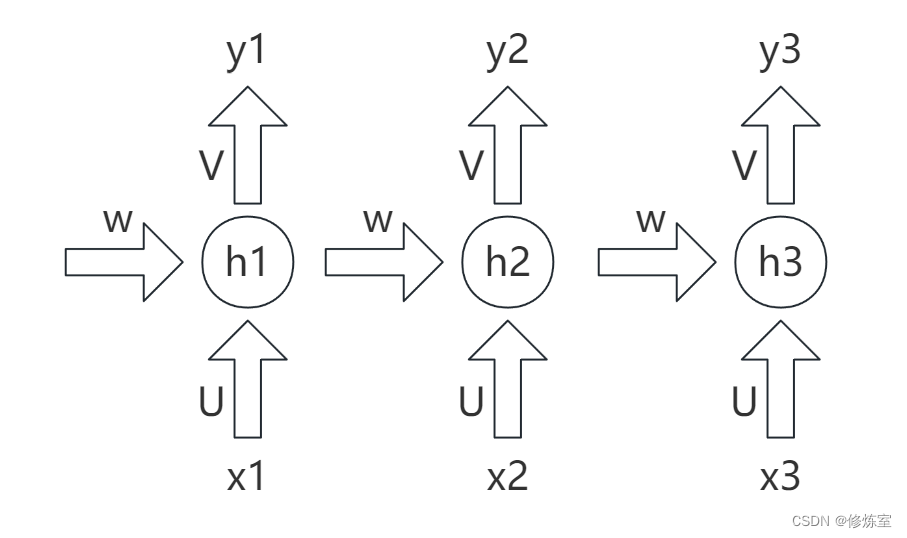
\includegraphics[width=1\textwidth]{../Pic/pic1.png} % Replace "example-image" with your image file
    \caption{Unfolded RNN}
\end{figure}

\newpage
\begin{longtable}{|c|c|c|}
    \hline
    \textbf{Notation} & \textbf{Meaning} & \textbf{Dimension}\\
    \hline
    $U$          & Weight matrix for input to hidden state       & $input\ size\times hidden\ unites$\\
    $W$          & Weight matrix for hidden to hidden state      & $hidden\ units\times hidden\ unites$\\
    $V$          & Weight matrix for hidden state to output state& $hidden\ units\times number\ of\ class$\\
    $x_t$        & Input vector at time t                        & $input\ size\times 1$\\
    $h_t$        & Hidden state output at time t                 & $hidden\ units\times 1$\\
    $b_h$        & Bias term for hidden state                    & $hidden\ units\times 1$\\
    $b_y$        & Bias term for output state                    & $number\ of\ class\times 1$\\
    $\hat{o}_y$  & Output at time t                              & $number\ of\ class\times 1$\\
    $\hat{y}_t$  & Output at time t                              & $hidden\ units\times 1$\\
    $\mathcal{L}$& Loss at time t                                & $scalar$\\
    \hline
    \caption{Unfolded RNN}
\end{longtable}
% Forward pass
\noindent \textbf{Forward Pass}
\\[1ex]
During the forward pass, the RNN processes the input sequence sequentially, computing hidden states and output at each timestep:
\begin{equation}
    h_t = f(U^Tx_{t}+W^Th_{t-1}+b_h)
\end{equation}
\begin{equation}
    \hat{y}_t = f(V^Th_t+b_y)
\end{equation}
\newline  % Computing the loss function
\noindent \textbf{Computing the loss function}
\\[1ex]
Assuming the loss is computed only at the final timestep t:
\begin{equation}
    \mathcal{L}_t = L(y_t, \hat{y}_t)
\end{equation}
In order to do backpropagation through time to tune the parameters in RNN, we need to calculate the partial derivative of loss function $\mathcal{L}$ with respect to the differently parameters.\\
\newline  % Backward pass using the chain rule
\noindent \textbf{Backward pass using the chain rule}
\\[1ex]
Using the chain rule for computing the gradient.\\
Partial derivative of loss function $\mathcal{L}$ with respect to $W$ (hidden to hidden state) at time 2. 
\begin{equation}
    \dfrac{\partial\mathcal{L}_2}{\partial W} = \dfrac{\partial\mathcal{L}_2}{\partial y_2} \cdot \dfrac{\partial y_2}{\partial h_2} \cdot \dfrac{\partial h_2}{\partial h_1} \cdot \dfrac{\partial h_1}{\partial W}
\end{equation}
By mathematic induction 
\begin{equation}
    \dfrac{\partial\mathcal{L}_t}{\partial W} = \dfrac{\partial\mathcal{L}_t}{\partial y_t} \cdot \dfrac{\partial y_t}{\partial h_t} \cdot (\sum_{i=1}^{t} \dfrac{\partial h_t}{\partial h_i} \cdot \dfrac{\partial h_i}{\partial W})
\end{equation}
Where 
\begin{equation}
    \dfrac{\partial h_t}{\partial h_i} = \prod_{j=i+1}^{t} \dfrac{\partial h_j}{\partial h_{j-1}}
\end{equation}

Partial derivative of loss function $\mathcal{L}$ with respect to $U$ (input to hidden state) at time 2.\\
\begin{equation}
    \dfrac{\partial\mathcal{L}_2}{\partial U} = \dfrac{\partial\mathcal{L}_2}{\partial y_2} \cdot \dfrac{\partial y_2}{\partial h_2} \cdot \dfrac{\partial h_2}{\partial h_1} \cdot \dfrac{\partial h_1}{\partial U}
\end{equation}
By mathematic induction 
\begin{equation}
    \dfrac{\partial\mathcal{L}_t}{\partial U} = \dfrac{\partial\mathcal{L}_t}{\partial y_t} \cdot \dfrac{\partial y_t}{\partial h_t} \cdot (\sum_{i=1}^{t} \dfrac{\partial h_t}{\partial h_i} \cdot \dfrac{\partial h_i}{\partial U})
\end{equation}
Where 
\begin{equation}
    \dfrac{\partial h_t}{\partial h_i} = \prod_{j=i+1}^{t} \dfrac{\partial h_j}{\partial h_{j-1}}
\end{equation}

Partial derivative of loss function $\mathcal{L}$ with respect to $V$ (hidden to output state) at time 2.\\
\begin{equation}
    \dfrac{\partial\mathcal{L}_2}{\partial V} = \dfrac{\partial\mathcal{L}_2}{\partial y_2} \cdot \dfrac{\partial y_2}{\partial h_2} \cdot \dfrac{\partial h_2}{\partial h_1} \cdot \dfrac{\partial h_1}{\partial V}
\end{equation}
By mathematic induction 
\begin{equation}
    \dfrac{\partial\mathcal{L}_t}{\partial V} = \dfrac{\partial\mathcal{L}_t}{\partial y_t} \cdot \dfrac{\partial y_t}{\partial h_t} \cdot (\sum_{i=1}^{t} \dfrac{\partial h_t}{\partial h_i} \cdot \dfrac{\partial h_i}{\partial V})
\end{equation}
Where 
\begin{equation}
    \dfrac{\partial h_t}{\partial h_i} = \prod_{j=i+1}^{t} \dfrac{\partial h_j}{\partial h_{j-1}}
\end{equation}

Partial derivative of loss function $\mathcal{L}$ with respect to $b_h$ (bias term in hidden state) at time 2.\\
\begin{equation}
    \dfrac{\partial\mathcal{L}_2}{\partial b_b} = \dfrac{\partial\mathcal{L}_2}{\partial y_2} \cdot \dfrac{\partial y_2}{\partial h_2} \cdot \dfrac{\partial h_2}{\partial h_1} \cdot \dfrac{\partial h_1}{\partial b_h}
\end{equation}
By mathematic induction 
\begin{equation}
    \dfrac{\partial\mathcal{L}_t}{\partial b_h} = \dfrac{\partial\mathcal{L}_t}{\partial y_t} \cdot \dfrac{\partial y_t}{\partial h_t} \cdot (\sum_{i=1}^{t} \dfrac{\partial h_t}{\partial h_i} \cdot \dfrac{\partial h_i}{\partial b_h})
\end{equation}
Where 
\begin{equation}
    \dfrac{\partial h_t}{\partial h_i} = \prod_{j=i+1}^{t} \dfrac{\partial h_j}{\partial h_{j-1}}
\end{equation}

Partial derivative of loss function $\mathcal{L}$ with respect to $b_y$ (bias term in output state) at time 2.
\begin{equation}
    \dfrac{\partial\mathcal{L}_2}{\partial b_y} = \dfrac{\partial\mathcal{L}_2}{\partial y_2} \cdot \dfrac{\partial y_2}{\partial h_2} \cdot \dfrac{\partial h_2}{\partial h_1} \cdot \dfrac{\partial h_1}{\partial b_y}
\end{equation}
By mathematic induction 
\begin{equation}
    \dfrac{\partial\mathcal{L}_t}{\partial b_y} = \dfrac{\partial\mathcal{L}_t}{\partial y_t} \cdot \dfrac{\partial y_t}{\partial h_t} \cdot (\sum_{i=1}^{t} \dfrac{\partial h_t}{\partial h_i} \cdot \dfrac{\partial h_i}{\partial b_y})
\end{equation}
Where 
\begin{equation}
    \dfrac{\partial h_t}{\partial h_i} = \prod_{j=i+1}^{t} \dfrac{\partial h_j}{\partial h_{j-1}}
\end{equation}

\textbf{parameters updates}
\begin{equation}
    W \leftarrow W - \alpha\dfrac{\partial\mathcal{L}}{\partial W}
\end{equation}
\begin{equation}
    U \leftarrow U - \alpha\dfrac{\partial\mathcal{L}}{\partial U}
\end{equation}
\begin{equation}
    V \leftarrow V - \alpha\dfrac{\partial\mathcal{L}}{\partial V}
\end{equation}
\begin{equation}
    b_h \leftarrow b_h - \alpha\dfrac{\partial\mathcal{L}}{\partial b_h}
\end{equation}
\begin{equation}
    b_y \leftarrow b_y - \alpha\dfrac{\partial\mathcal{L}}{\partial b_y}
\end{equation}

\textbf{Pseudocode of BPTT} \parencite{wikipedia2023bptt}
\begin{algorithm}[H]
    \caption{Backpropagation Through Time (BPTT)}
    \begin{algorithmic}[1]
    \STATE \textbf{Input:} 
    \STATE \hspace{1em} Sequence of input data $\{x_1, x_2, \dots, x_T\}$
    \STATE \hspace{1em} Sequence of target outputs $\{y_1, y_2, \dots, y_T\}$
    \STATE \hspace{1em} Learning rate $\eta$
    \STATE \hspace{1em} Number of time steps to unroll $N$
    \STATE \textbf{Initialize:} Model parameters $\theta$, hidden state $h_0 = 0$
    
    \STATE \textbf{Forward Pass:}
    \FOR{$t = 1$ to $T$}
        \STATE Compute hidden state: $h_t = f(h_{t-1}, x_t; \theta)$
        \STATE Compute output: $\hat{y}_t = g(h_t; \theta)$
        \STATE Compute loss for time step $t$: $L_t = \mathcal{L}(\hat{y}_t, y_t)$
    \ENDFOR
    
    \STATE \textbf{Backward Pass (BPTT):}
    \STATE Set total loss: $L = \sum_{t=1}^{T} L_t$
    \FOR{$t = T$ down to $1$}
        \STATE Compute gradient of loss with respect to output: $\frac{\partial L_t}{\partial \hat{y}_t}$
        \STATE Backpropagate through output layer to obtain: $\frac{\partial L_t}{\partial h_t}$
        \STATE Accumulate gradients for parameters: $\frac{\partial L}{\partial \theta}$
        \FOR{$k = 1$ to $N$}
            \STATE Backpropagate through time for $N$ steps:
            \STATE Compute gradient contribution from step $t-k$: $\frac{\partial L_t}{\partial h_{t-k}}$
        \ENDFOR
    \ENDFOR
    
    \STATE \textbf{Update Parameters:}
    \STATE $\theta = \theta - \eta \cdot \frac{\partial L}{\partial \theta}$
    
    \STATE \textbf{Output:} Updated parameters $\theta$
    \end{algorithmic}
\end{algorithm}

\newpage
% Actication function
\subsubsection{Activation Function}
Activation functions, particularly the sigmoid function, are fundamental components of recurrent neural networks (RNNs). They transform input data into output data. A key property of these functions is their differentiability. Differentiability is crucial for the backpropagation through time (BPTT) algorithm, enabling the application of the chain rule during training. \\[1ex]
% Sigmoid Activation Function 
\textbf{Sigmoid activation function}
\\[1ex]
The main role of the sigmoid activation function is to normalize candidate values and convert the cell state to a hidden state when performing cell state updates. It limits the output between [0,1] because it has a smooth gradient, which is important for discovering long-range dependencies.\\[1ex]
\begin{equation}
    Sigmoid(x) = \frac{ 1 }{ 1+e^{-x} }
\end{equation}
\begin{equation}
    Sigmoid'(x) = Sigmoid(x)(1-Sigmoid(x))
\end{equation}
Below is the sigmoid function and its derivative.
\begin{figure}[!htb]
    \centering
    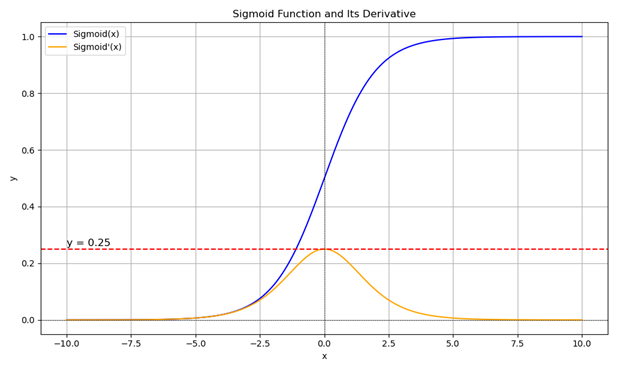
\includegraphics[width=1\textwidth]{../Pic/sigmoid.png} % Replace "example-image" with your image file
    % \caption{An example image.}
    \label{fig:sigmoid}
\end{figure}
\newline
$Domain(Sigmoid(x))=\mathbb{R},\hspace{1em} Codomain(Sigmoid(x))=(0,1)$\\
$Domain(Sigmoid'(x))=\mathbb{R},\hspace{1em} Codomain(Sigmoid'(x))=[0,0.5]$

% Hyperbolic tangent activation function
\newpage
\textbf{Hyperbolic tangent activation function}
\\[1ex]
The main role of the hyperbolic tangent (tanh) activation function is to normalize candidate values and convert the cell state to a hidden state when performing cell state updates. It limits the output between [-1,1] because it has a stable gradient, which is important for discovering long-range dependencies.
\newline
\begin{equation}
    tanh(x) = \frac{ e^{x} - e^{-x} }{e^{x} + e^{-x}}
\end{equation}
\begin{equation}
    tanh'(x) = 1 - tanh^{2}(x)
\end{equation}
Below is the Hyperbolic tangent activation function and its derivative.\\
\begin{figure}[!htb]
    \centering
    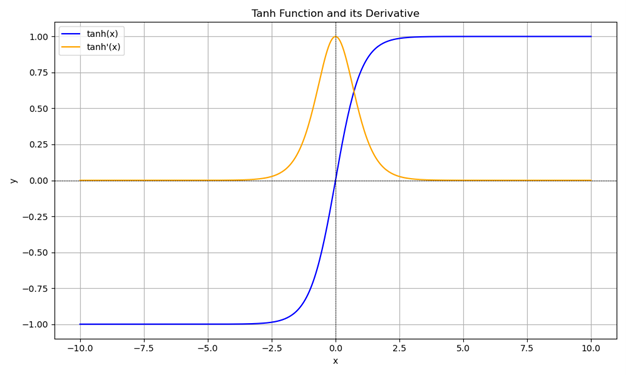
\includegraphics[width=1\textwidth]{../Pic/tanh.png} % Replace "example-image" with your image file
    % \caption{An example image.}
    \label{fig:tanh}
\end{figure}
\newline
$Domain(tanh(x))=\mathbb{R},\hspace{1em} Codomain(tanh(x))=[-1,1]$\\
$Domain(tanh'(x))=\mathbb{R},\hspace{1em} Codomain(tanh'(x))=[0,1]$

% Gradient vanishing and gradient exploring
\newpage
\textbf{Gradient vanishing and gradient exploring}
\\[1ex]
When training the RNN, BPTT was used to update the weight matrix. As the number of time steps increase, the problem of gradient instability of often encountered, and this problem is gradient vanishing and gradient explored \parencite{bengio1994learning}. 
\\[2ex]
% Vanishing Gradients
\textbf{Vanishing Gradients}
\\[1ex]
Generally, sigmoid activation function is used commonly in RNNs, has a maximum derivative of 0.25. When doing BPTT in long time steps, this multiplication results in exponentially diminishing gradients as the sequence length increases. Consequently, the shallow neural receive very small gradient updates, making it difficult to adjust the parameters effectively. This leads to the model struggling to learn long time dependencies. 
\\[1ex]
% Exploding Gradients
\textbf{Exploding Gradients}
\\[1ex]
When we are doing the feedforward and get super large value computed by loss function. Then when updating the parameters. The updates to the weights will also be large. Resulting in higher loss and larger gradients in the next iterations. This will lead to exploding gradients.
\\[1ex]
We have introduce the backpropagation through time. This is the method to update the parameters in RNNs. When calculating, for example, the partial derivative of loss function with respect to W. Assume the time $t$ go to infinity large. We will get this term. $ \prod_{j=i+1}^{t} \dfrac{\partial h_j}{\partial h_{j-1}} $, and it will lead to exponential problem. if $ \dfrac{\partial h_j}{\partial h_{j-1}} > 1 $. Then the product of all term will increase exponentially, then exploding gradients occur. On the contrary, if $\dfrac{\partial h_j}{\partial h_{j-1}} < 1$. Then the result will decrease exponentially, then vanishing gradients occur.

% ######################## Background and Literature Review #########################


\end{document}